\documentclass{article}
\usepackage{mathtools}
\usepackage{csquotes}
\renewcommand{\baselinestretch}{1.2} 
\newcommand{\eg}{{\em e.g., }}


\usepackage{Sweave}
\begin{document}

\begin{centering}
\huge{MBITES}\\
\vspace{0.3in}
\Large{Mosquito Bout-based and Individual-based \\ Transmission Ecology Simulator}\\

\vspace{0.3in}
\large{MBITES Development Team: \\ Sean Wu, Hector Sanchez, Qian Zhang, John Henry, Daniel Citron, Amit Verma, Arnaud Le Menach, David L Smith\\}

\end{centering}

%\newcommand{\mbites}{{\cal MBITES}}

\Sconcordance{concordance:MBITES-Supplement.tex:MBITES-Supplement.Rnw:%
1 7 1 1 0 142 1 1 36 38 0 1 2 74 1 1 9 11 0 1 2 247 1 1 16 18 0 1 2 19 %
1 1 7 1 2 4 1 1 23 1 4 13 1 1 14 16 0 1 2 13 1}


\paragraph{Introduction}

\begin{displayquote}
{\bf \em What is MBITES?}
\end{displayquote}

This document is a users guide to MBITES (Mosquito Bout-based and Individual-based Transmission Ecology Simulator), a software package for simulating mosquito-borne pathogen transmission and vector control. 

MBITES is comprised of several parts: a {\bf landscape} describing resources used by adult mosquitoes; the algorithms describing adult behavior as a sequence of flight {\bf bouts}; a set of configurable {\bf options} for simulating other aspects of mosquito life-history and behavior; {\bf vector control}; and the aquatic ecology. MBITES also includes functionality for simulating pathogen transmission as part of a larger software package called MASH (Modular Analysis through Simulation of human Health). 

The following five sections describe these parts of MBITES. Each section begins with a brief summary or
heuristic followed by implementation notes, relevant details, and a guide to the R code. 


\paragraph{The MASH Framework}

\begin{displayquote}
{\em {\bf NOTE:} The following section gives some background and vocabulary for understanding some of the basic concepts and design principles of MASH and MBITES. We recommend reading it at some point, but feel free to skip it.}
\end{displayquote}

MBITES is a flexible module that runs the adult mosquito component of MASH. The terms ``component,''``module,'' and ``flexible'' all have a specific meaning in MASH. The following section explains the terminology used in MBITES and MASH and the rationale for developing it.  

MASH is a framework for simulating human health events and related phenomena (\eg pathogen transmission by mosquito populations). MASH is a simulation modeling framework, not a simulation model. To put it another way, the problem MASH was trying to solve was how to build a plug-and-play simulator for human health, not how to simulate human health. The core design problem for MASH was how to build an API (application program interface) defining how various components of a model interact. The philosophy of MASH was that every component should have at least two modules: one would be highly realistic and simulate the relevant phenomena in exquisite detail, and the other would be dead simple. The first disease to be implemented within MASH was malaria. 

The collection of all mechanistic models of human malaria have the same basic structural parts: a model of human malaria infection and immunity; a model of mosquito populations, including infection and development of malaria parasites; and some model of immature mosquito  populations in their aquatic habitats. In MASH, each one of these parts is called a \verb1COMPONENT1. Four distinct biological processes determine how these three components interact: malaria parasites can be passed from mosquitoes to infect humans when mosquitoes probe in anticipation of taking a blood meal; parasites infecting humans can be passed in the blood meal, infecting mosquitoes; adult mosquitoes lay eggs in aquatic habitats; and the eggs hatch, develop through four larval instars, then pupate and emerge as imago (the mature form) from the aquatic habitats to begin their lives as volant adults. A structure allowing MASH components to interact is called a \verb1QUEUE1. In its most general form, transmission describes the events when pathogens are transmitted, either from mosquitoes to humans or {\em vice versa}, but it also the dispersion of pathogens, the distances traveled by the pathogens between infection events. The \verb1LANDSCAPE1 is the part of the model that determines how dispersion is defined. 

To be truly plug-and-play, it must be possible to represent any other component trivially as a parameter, which is what we have done here. MBITES is the exquisitely detailed module for simulating the blood feeding behavior of adult mosquito populations. This document also describes how MBITES is coupled to the component describing the aquatic ecology. We describe how MBITES can be used to simulate pathogen transmission among populations of humans and mosquitoes; here we describe how that would happen without actually simulating transmission.  

The structure of MASH is summarized in the following way:
\begin{itemize}
\item MASH Structure
  \begin{itemize}
  \item A population of \verb1HUMANS1 and their health states and health events is the core of MASH. 
  \item A \verb1COMPONENT1 is a basic functional part of any human health model. 
  \item A \verb1LANDSCAPE1 defines the spatial scaffold for interactions. 
  \item A \verb1QUEUE1 is a component level structure allowing two distinct components to interact. 
  \end{itemize} 
\item A \verb1Module1 is a specific set of algorithms that instantiates a component. A module could be flexible in the sense that the same process could be represented by one of many different functional forms. 
\item A \verb1Synthetic Population1 is the fully configured set of initial conditions.  
\end{itemize}
%
MASH is a framework for building models that is modular and flexible. 

This gives rise to a complementary vocaublary to describe the models that arise. We consider MBITES to be a CLASS of models: 
\begin{itemize}
\item Two models belong to the same ORDER if they belong to the same CLASS and share the same state space. 
\item Two models belong to the same FAMILY if they belong to the same ORDER and use the same functional forms.
\item Two models belong to the same GENUS if they belong to the same FAMILY and share the same parameters.
\item Two models belong to the same SPECIES if they belong to the same GENUS and share the same synthetic population.
\item An individual model is an individual member of a SPECIES defined by its random number seed. 
\end{itemize}
%
Species-level similarity is the default meaning of {\em \bf model} in MASH. Without some explicit way of mapping the state space, it is difficult to compare two models belonging to a different order. This nomenclature system (borrowed from Linnaeus) makes it possible to talk about models defined by some other level of similarity (\eg model families).

\section{Landscape}

MBITES uses a landscape structure called \verb1MICRO1.  We think of a \verb1MICRO1 landscape as being comprised of different point sets on which mosquito activities occur: 
%
\begin{itemize}
\item[f] :: haunts or blood feeding sites where feeding occurs
\item[l] :: habitats, short for aquatic habitats where egg laying occurs
\item[s] :: sugar, or sites where sugar feeding occurs
\item[m] :: mating sites
\end{itemize}
%
In MBITES, blood feeding is an event that occurs only at a blood feeding site, which typically include all the houses and other dwellings where people live. Another set of points describes where humans go to seek care:
%
\begin{itemize}
\item[c] :: clinics or community health workers
\end{itemize}
%
While this is the way we think about landscapes, there is in fact one master point set where {\em any} events happen, and each unique point is called a {\em site}. A set of boolean switch describes the kinds of events (\eg blood feeding, egg laying, sugar feeding, mating, or care seeking) occurring there.  

Each site is determined by a location in space ($x,y$), and it has a {\em site type}, which determines how mosquitoes rest (\eg around a homestead; \verb1restingSpot()1 is described in Options : Resting Hazards). 

There are also other properties of each site. Each site has a pair of numbers that determine its location $(x,y)$. Each type of function ($*$) has a search weight associated with it for each species: $\omega_{i, *}$. 

The main point of a landscape is to provide a template upon which different components of the model can interact. Humans and mosquitoes interact mainly through blood feeding, but for this to occur, there must be a way for humans and mosquitoes to meet up on the landscape.  The structures that allow for components to interact are called queues. 

\subsection{Configuring a Landscape}



\section{Mosquito Bouts}

A mosquito bout tracks a mosquito from its launch to initiate one bout up to the point when it launches itself to initiate the next bout. Conceptually, the structure of a bout is:  {\bf Launch} - {\bf Try} - {\bf Land} - {\bf Rest}. The {\bf Try} part of the bout is found in code \verb1boutX1 where \verb1X1 is one of the following: 
\begin{itemize}
\item[F] :: A search to find a place where blood feeding can occur
\item[B] :: An attempt to blood feed on a host that is present
\item[R] :: The post-prandial resting bout
\item[L] :: A search to find a place where egg laying can occur
\item[O] :: An attempt to lay eggs
\item[M] :: Mating, which could include a search flight 
\item[S] :: Sugar feeding, which could include a search flight 
\end{itemize}
%
After the bout, a mosquito lands at a particular kind of place, determined by the function \verb1restingSpot()1. The mosquito's energetic state is then updated, with \verb1sugarEnergetics()1.

Mortality can occur as a result of flight stress or from one of the many hazards during landing. At the end, survival is computed by their associated functions: \verb1surviveResting()1 and \verb1surviveFlight()1.

Finally, every mosquito event is logged through \verb1historyTrack()1. 

\paragraph{Implementation Notes}

All bouts are implemented within a generic bout framework, in the function \verb1mbites_oneBout()1.

In computing the outcome of a flight bout, variables track the  event times (\verb1tNow1, and \verb1tNext1) -- the moment when it started the bout; the mosquito's location among the point sets (\verb1locNow1, and \verb1locNext1); and the mosquito's present and future state (\verb1state1, and \verb1stateNew1). Before starting a new flight bout, \verb1tNext1 has been checked to be sure other dependent elements of the simulation have been correctly set. 
Upon entering the bout, the mosquitoes time, state, and location are updated:
\begin{itemize}
\item \verb1tNow = tNext1
\item \verb1tNext = timing()1
\item \verb1locNow = locNext1
\item \verb1locNext = moveMe()1
\item \verb1state = stateNew1
\end{itemize}
The \verb1state1 ($=$\verb1X1) determines which kind of bout occurs; \verb1boutX1 is run, setting \verb1stateNew1. 

To avoid errors caused by updating \verb1state1 at the wrong time, all calculations within a bout use the {\em present} time, location, and state: \verb1tNow1, \verb1state1, and \verb1locNow1. 

To avoid resurrecting a dead mosquito or resuscitating an estivating mosquito, any code that could change a mosquito's behavioral state is run only if the function \verb1isActive()1 returns \verb1TRUE1. 




\paragraph{R-Code}
\begin{Schunk}
\begin{Sinput}
> mbites_oneBout <- function(){
+ 
+   # update time and state
+   private$tNow = private$tNext # update time
+   private$state = private$stateNew # update current state
+   self$timing() # update tNext
+ 
+   # movement
+   self$moveMe()
+ 
+   # bout
+   switch(private$state,
+     F = {self$boutF()},
+     B = {self$boutB()},
+     R = {self$boutR()},
+     L = {self$boutL()},
+     O = {self$boutO()},
+     M = {self$boutM()},
+     S = {self$boutS()},
+     {stop(cat("illegal behavioral state: ",private$state,"\n",sep=""))}
+   )
+ 
+   # landing spot
+   self$restingSpot()
+ 
+   # energetics
+   self$sugarEnergetics()  # MBITES-Generic-Energetics.R
+ 
+   # survival
+   self$surviveResting()     # MBITES-Generic-Survival.R
+   self$surviveFlight()      # MBITES-Generic-Survival.R
+ 
+   # log history
+   private$history$historyTrack(privateEnv = private, alive = self$isAlive())
+ }
\end{Sinput}
\end{Schunk}


\subsection{Blood Feeding Search Bout [F]}

If a female mosquito is not in the neighborhood of a blood meal host, she must search for one. She might also initiate a new search bout, even if the site she occupies is suitable for blood feeding. In some cases, such as peri-domestic breeding, where it is not necessary to move to find a bloodmeal host, she might initiate a blood feeding attempt bout without a blood meal search bout. 

A flight search bout for blood feeding could begin anywhere, but
it always ends at a {\em feeding site} or {\em haunt}:
%
\begin{equation}
%
\left\{  l \right\}
\cup
\left\{  f \right\}  \cup \ldots
\overset{{\cal K}_F}{\rightarrow}
\left\{  f \right\}
%
\end{equation}
%
The outcome of a search bout is either mosquito death, a new
(possibly the same) location and behavioral state, or a
frustrated search attempt without a change of behavioral state.

The function ${\cal K}_F$ is implemented by \verb1rMove()1, described in the options below. 

\paragraph{Implementation}

\begin{itemize}
%
\item The function \verb1rMove()1 is called to determine the mosquito's next location. 
%
\item A parameter, \verb1bfsb.s1, determines whether a mosquito
has a ``success'' on its approach to the haunt. If the flight was
a ''success,'' then its behavioral state is set to {\bf B}.
Otherwise, it remains in state {\bf F}.
%
\item The function  \verb1restingSpot()1 is then called. A
mosquito can fail to find a suitable resting place and thus
decided to leave (denoted \verb1bfrs.f1) in which case its
behavioral state is set to {\bf F}.
%
\item The function  \verb1sugarEnergetics()1 is then called. A
mosquito can fail to find a suitable resting place and thus
decided to leave (denoted \verb1bfrs.f1) in which case its
behavioral state is set to {\bf F}.
%
\item The functions \verb1surviveFlight()1 is then called, which
computes the probability of surviving the flight, \verb1bfsb.fs1.
If a mosquito dies, its state is set to {\bf D}.
%
\item The functions \verb1surviveResting()1 is then called, which
computes the probability of surviving from landing through
launch, \verb1bfsb.rs1. If a mosquito dies, its state is set to
{\bf D}.
%
\end{itemize}

\paragraph{Transition Probabilities}

The mosquito's ending state is:

\begin{itemize}
\item[{\bf D}] with probabilty $P_{FD} = 1 - $\verb1bfsb.fs1 $\times$
\verb1bfsb.rs1
\item[{\bf F}] with probability $P_{FF} = (1-P_{FD}) ($\verb1bfrs.f1 $+
(1-$\verb1bfrs.f1$)(1-$\verb1bfsb.s1$))$.
\item[{\bf B}] with probability $P_{FB} = 1-P_{FF}$.
\end{itemize}

\paragraph{R-Code}


\begin{Schunk}
\begin{Sinput}
> mbites_boutF <- function(){
+   if(private$lspot != "l" & runif(1) < 
+      private$FemalePopPointer$get_MBITES_PAR("F_succeed")){
+     private$stateNew = "B"
+   } else {
+     private$stateNew = "F"
+   }
+ }
\end{Sinput}
\end{Schunk}

\subsection{Blood Feeding Attempt Bout [B]}

A blood feeding bout begins when a mosquito chooses a host to
approach. Information about the human hosts present in each haunt
are stored in a queue, called {\em atRisk}. Other potential blood
meal hosts (\eg cattle) can also be present. Each host has a
weight, which is used in a multinomial probability distribution
function to select one of the hosts to approach.

After selecting a host, different functions determine the outcome
of an attempt, depending on whether the host is human or another
vertebrate animal. As a mosquito approaches a human attempting to
blood feed, there are several steps: an approach, probing, and
the blood meal. The mosquito could be frustrated or killed at
each one of these steps (\eg from swatting). A mosquito blood
feeding on a human becomes infected with a pathogen with some
probability. Pathogens mature by a (possibly temperature
dependent) rule determining EIP at some point in the future, if
the mosquito is still alive.

The process for feeding on a non-human vertebrate animals is
simpler; parameters determine the probability of death or success
(and their complement, failure followed by a new attempt).

After successfully blood feeding, a mosquito's behavioral state
changes to the post-prandial resting bout. If a mosquito survives
the attempt but does not succeed in taking a blood meal, then it
can either repeat a blood feeding attempt or leave the area to
search for a new site.

If a mosquito has successfully blood fed, a random variate is
drawn to determine the size of the blood meal, and there is
another function that determines whether the mosquito survives
the stress associated with blood feeding, depending on the size
of the blood meal.

\paragraph{Post Prandial Resting Bout [R]}

The outcome of a post prandial resting bout is either death,
another attempt to blood feed, or an egg laying search bout.

Transition to egg laying behaviors depends on a rule determining
how eggs mature, depending on the time required for egg
maturation {\em vs.} the time required for a feeding bout. If egg
maturation occurs every feeding bout, then blood is provisioned
into eggs; the larger the blood meal, the larger the egg batch. A
mosquito could choose to feed again, depending on the size of the
blood meal / egg batch. Another option is that the eggs require
time or blood resources to mature. If eggs are maturing, a
mosquito repeats a blood feeding attempt until the eggs are
mature.

If a mosquito survives, but the eggs are not mature or if she
decides to top-up, she will attempt another blood meal. Even if
eggs are mature, the mosquito may attempt to blood feed again,
depending on the size of the last bloodmeal. Otherwise, a
surviving mosquito makes an attempt to lays eggs.

\paragraph{Egg Laying Search Bout [L]}

A female mosquito must search for an egg laying habitat, though
(as in the case of peri-domestic breeding) one might be readily
available. In such cases, the ``search'' results only in a change
of state. A flight search bout for blood feeding could begin
anywhere, but it always ends at a haunt:
%
\begin{equation}
%
\left\{ l\right\}  \cup \left\{ f\right\}
\overset{L}{\rightarrow} \left\{ l\right\}
%
\end{equation}
%
The outcome of a search bout is either mosquito death, success
and a change of location and behavioral state, or a frustrated
search attempt with a change of location but without changing
behavioral state. In some cases, such as peri-domestic breeding,
where a mosquito finds herself already in an egg laying site, the
mosquito might bypass an egg laying search flight.

\paragraph{Egg Laying Attempt Bout [O]}

An egg laying bout involves a series of egg laying attempts where
a mosquito dies, successfully lays some fraction of the eggs and
initiates a new egg laying search bout, or is frustrated. If
frustrated, she will either either make another attempt to lay
eggs or initiate a new attempt somewhere else.


\paragraph{Maturation}

\paragraph{Male Mosquito Populations}

\paragraph{Mating Bouts and Maturation}

Mating requires simulating male mosquito populations. MBITES can
simulate both female and male individuals. After an adult female
has emerged from her pupal case and hardened, she is considered
to be {\em pre-gonotrophic}. The conditions for maturation
include a mating requirement and (possibly) an energetic
requirement, meaning that she could not lay eggs until she had
mated and satisfied an early life energy intake requirement. The
model has not pre-determined what these pre-gonotrophic energetic
requirements are, but provides a flexible set of functions and
parameters to stipulate, depending on the species and either
evidence or expert opinion. Mating and maturation can also be
turned off, such that a female is mature and mated upon
emergence.

Male mosquitoes emerge from aquatic habitats and by default
attempt to sugar feed (see below). At a specific time of each
day, the male behavioral state switches to {\bf M}, and it moves
to a mating point, $\left\{ m \right\}$, to be present for any
female arriving at that point to mate.
Male search thus always begins at a mating or sugar feeding site,
$\left\{ s \right\} $ to arrive at a mating site $\left\{ m
\right\}$:
%
\begin{equation}
%
\left\{ s\right\} \cup \left\{ m\right\}  \overset{{\cal
K}_M}{\rightarrow} \left\{ m\right\}
%
\end{equation}
%
If the male mosquito survives the flight, it enters a swarm. The
{\em swarming queue} tracks all the male mosquitoes present at
each point in $\left\{ m\right\} $ on each day. After the swarm
disperses, surviving males behavioral states switch back to {\bf
S} to sugar feed (see below).

A pre-gonotrophic female does not lay eggs, though she can blood
feed. Female mating bouts in this model occur only when she is in
a pre-gonotrophic state, which (like males) can be triggered
during a specific time window each day, when her state switches
to {\bf M}. The female search kernel could thus begins at any
mating, blood feeding, or sugar feeding site but always ends at a
mating site $\left\{ m\right\} $:
%
\begin{equation}
%
\left\{ f\right\} \cup \left\{ s\right\} \cup \left\{ m\right\}
\overset{{\cal K}_M}{\rightarrow} \left\{ m\right\}
%
\end{equation}
%
A female chooses from among the males in the queue at that
location. The probability of success is a function of the number
of males present in the swarm. When a female mosquito mates, the
identity of the male mosquitoes she mated with are chosen from
those present at the swarming site and stored. The outcome of a
mating bout is either death, success, or failure. After a mating
bout, a female's behavioral state switches to search for a blood
meal, {\bf F}.

An alternative to swarming behavior is opportunistic mating
during some other activity (\eg blood feeding). If males are
present where females blood feed, a random variate is drawn to
see if the blood feeding attempt bout is interrupted and mating
occurs. In such cases, ordinary hazards apply, and if the female
survives, her behavioral state does not change. (NOTE: we need to
add this possibility, just as we do for sugar feeding.)

\paragraph{Sugar Feeding Bouts and Energetics}

A variable track's the level of each mosquito's energy reserves,
and each bout depletes a mosquito's energy reserves by some
amount. These energy reserves could be restored by blood feeding,
depending on the species (a parameter is set to determine how
much energy a female mosquito is able to derive from blood).
Otherwise, a mosquito must restore its energy reserves by sugar
feeding. Sugar sources are distributed across the landscape, at
the points in $\left\{ s\right\} $, including possibly at
swarming sites, haunts, and habitats. Sugar feeding could occur
in two ways, through a sugar feeding bout or opportunistically.

A female mosquito's energy reserves are checked at the end of
every other kind of bout, and a function determines whether a
mosquito switches from some other state into an active sugar
feeding behavioral state, thereby initiating a sugar feeding
bout. A mosquito sugar feeding bout could begin at any haunt or
at another habitat, but it always ends in a sugar feeding site:
%
\begin{equation}
%
\left\{ f\right\} \cup \left\{ l\right\}  \cup \left\{ m\right\}
\cup \left\{ s\right\}  \overset{L}{\rightarrow} \left\{
s\right\}
%
\end{equation}
%
The outcome of a sugar bout is either death, a sugar meal, or
another attempt. If a sugar feeding bout succeeds, the sugar
reserves are topped up.

During any other kind of bout, opportunistic sugar feeding can be
triggered in a female if sugar is present. The functions
triggering obligate and opportunistic feeding are, by default,
shifted so that a female mosquito is more likely to feed
opportunistically than to actively sugar feed. The sugar reserves
of a mosquito are checked. The sugar at the source has a ``search
weight,'' and functions determine whether a mosquito chooses to
feed based on energy reserve levels and the weight. Another
function determines how much the reserves are topped up. If a
mosquito does sugar feed opportunistically, the mosquito could
die during the attempt. If it survives opportunistic feeding, its
behavioral state remains the same.

Male mosquitoes are obligate sugar feeders when they are not
mating. Sugar feeding will occur repeatedly until the time window
when mating occurs, when its state shifts back to mating.



\paragraph{Estivation [E]}

Estivation is a state of inactivity. In this model, estivation is
induced seasonally, whenever certain conditions are met (\eg no
rain). If a mosquito survives estivation, it initiates a blood
feeding search bout at some point in the future.

\section{Options}

Other properties of a site include a set of queues that coordinate information sharing from one \verb1COMPONENT1 to another. 

\subsection{Time at Risk}

\subsection{Egg Laying}

\subsection{Emergence}

\subsection{Mosquito Dispersal}

Mosquito dispersal occurs as the result of a search bout, called by the function \verb1rMove()1. 

\subsubsection{Kernels}

%\subsubsection{Kernels}


\subsection{Surviving the Flight}

When \verb1surviveFlight()1 is called, a random number is drawn
to determine whether the mosquito survived the stress associated
with flight. The function is called from {\bf
MBITES-GenericSurvival.R} and at the moment, it looks like this: 
%
\begin{Schunk}
\begin{Sinput}
> mbitesGeneric_surviveFlight <- function(){
+   if(self$isActive()){
+     p = self$get_surviveFlightProb()
+     if(private$FemalePopPointer$get_MBITES_PAR("TATTER")){
+       private$damage = private$damage + self$WingTattering()
+       p = p * self$pTatter()
+     }
+     if(private$FemalePopPointer$get_MBITES_PAR("SENESCE")){
+       p = p * self$pSenesce()
+     }
+     if(runif(1) < 1-p){
+       private$stateNew = "D"
+     }
+   }
+ }
\end{Sinput}
\end{Schunk}

\paragraph{Baseline Survival} 

The function \verb1get_surviveFlightProb()1 returns the
probability of surviving.  {\bf I can't find this function}   
 
\paragraph{Senescence}

Senescence is defined in this model as a reduction in the
probability of surviving that is associated with a  mosquito's
chronological age, $a$. In MBITES, senescence has been
implemented as an increased probability of mortality, per bite,
that increases with the chronological age of the mosquito when it
takes a flight bout. The function describing
the probability of surviving is 
%
$$\frac{2+sns.b}{1+sns.b} -
\frac{e^{a*sns.a}}{sns.b + e^{a*sns.a}}.  
$$ 
%
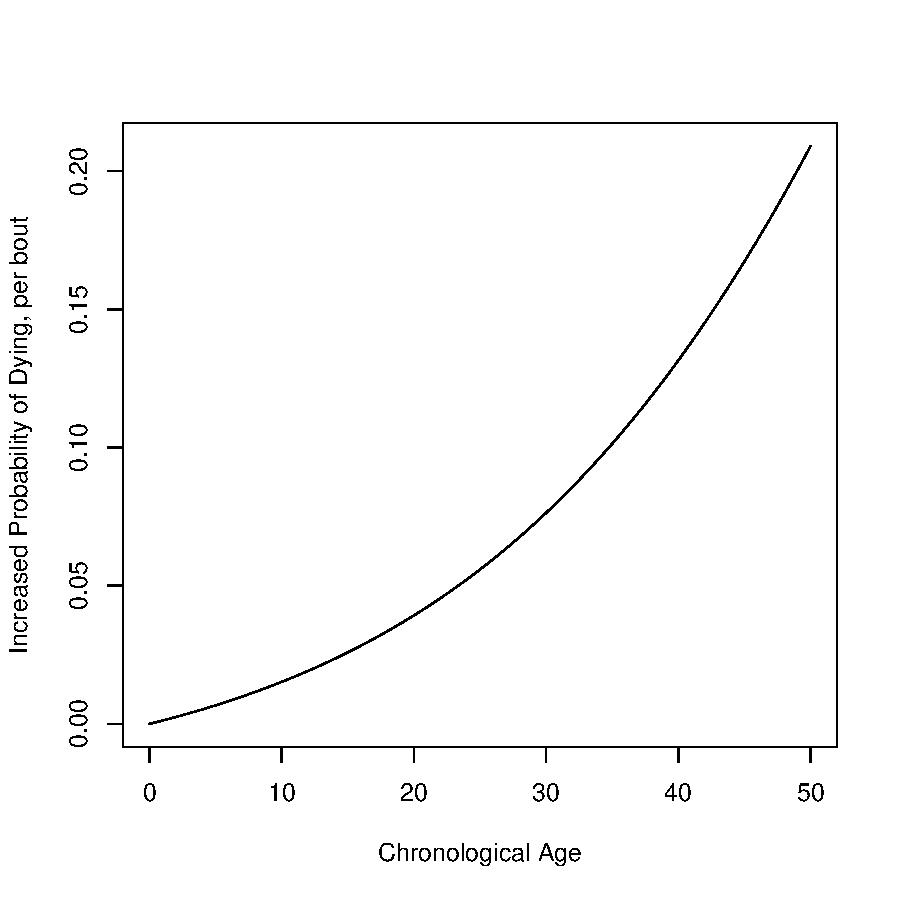
\includegraphics{MBITES-Supplement-004}

{\bf NOTE: overall survival vs. age is difficult to compute without simulation. 
It would be good for the GUI to show surival of ~1,000 mosquitoes with and without senescence, 
and to compute (and show) the average age. Something like this:}  

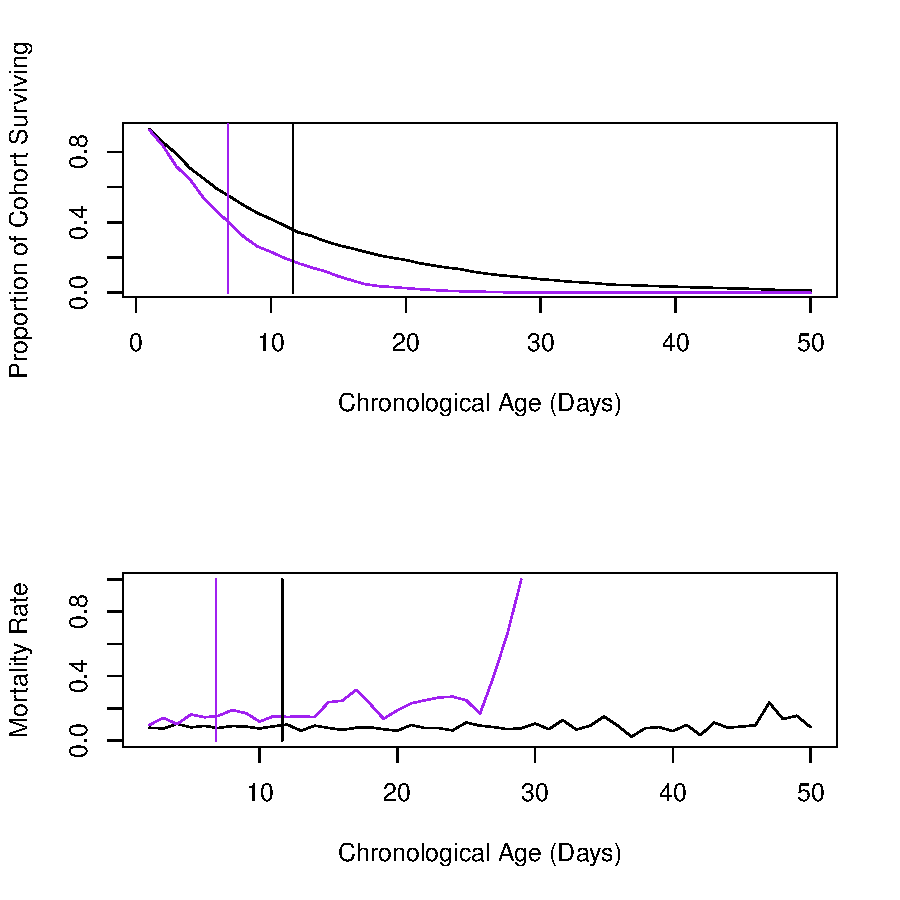
\includegraphics{MBITES-Supplement-005}

\paragraph{Wing Tattering}

\subsection{Resting Hazards}

This discusses implementation and options for \verb1surviveResting()1. One reason for determining where a host rests is for purposes of simulating various modes of vector control or entomological surveillance, including IRS, housing improvements, area repellants, eave tubes, or window traps.

\subsubsection{A Simple Site}

A simple type is given an index 


\paragraph{R Code}

\begin{Schunk}
\begin{Sinput}
> mbites_restingSpot <- function(){
+   if(self$isActive()){
+     if(self$searchFail()){
+       private$lspot = "l"
+     } else {
+       oldSpot = private$lspot
+       private$lspot = self$newSpot() # choose new lspot
+       if(oldSpot != "i" & private$lspot == "i"){
+         self$enterHouse() # enterHouse
+       }
+     }
+   }
+ }
\end{Sinput}
\end{Schunk}

\subsection{The Blood Meal}


\subsection{Time to Event} 



\section{Aquatic Ecology}




\end{document}
